\documentclass[text01.tex]{subfiles}
\begin{document}
%
% section 1.2
%
\section{ラズベリーパイになれよう（１）}

%
% subsection 1.2.1
%
\subsection{ファイルとフォルダ}

コンピュータやラズベリーパイの中にあるデータ（音楽、動画、写真、テキストなど）はすべてファイルとして\ruby{扱}{あつか}われています。
ファイルには.(ドット)から始まる「\ruby{拡張子}{かくちょうし}」がついています。
拡張子は、どんな種類のファイルかを表します。
例えば\ruby{画像}{がぞう}ファイルには.jpgや.png、動画ファイルには.mp4、テキストファイルには.txt、ホームページには.htmlなどが使われます。

ファイルの他にフォルダがあります。フォルダはファイルをまとめて\ruby{保存}{ほぞん}するための入れ物のようなものです。
ファイルを書類とすると、フォルダはそれをまとめるバインダに例えることができます。
フォルダの中にフォルダを入れることもできます。

\begin{figure}[hb]
  \centering
    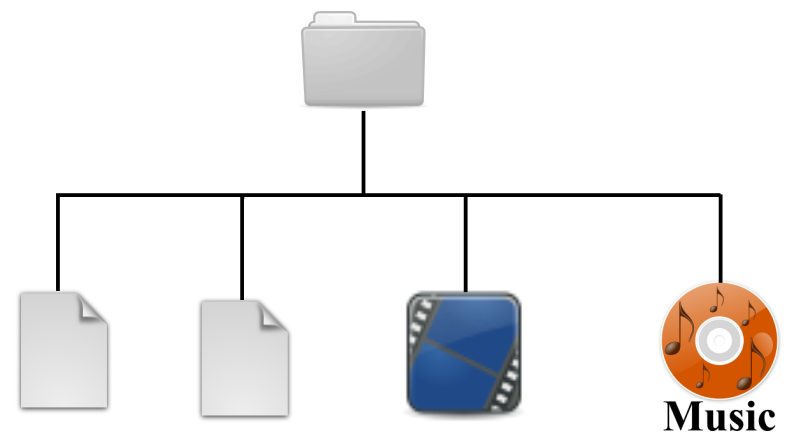
\includegraphics[keepaspectratio, height=50mm]{../../asset/image/figure15.png}
    \caption{フォルダとファイルの関係}
    \label{fig:19}
\end{figure}



%
% subsubsection 1
%
\subsubsection{自分のフォルダを\ruby{確認}{かくにん}しよう}
\hrule\vspace*{5mm}

まず、みなさんがこの\ruby{授業}{じゅぎょう}で使う「自分のフォルダ」を\ruby{確認}{かくにん}しましょう。
さきほど、みなさんには「ユーザ名」と「パスワード」を\ruby{設定}{せってい}してもらいました。
そのとき\ruby{設定}{せってい}した「ユーザ名」によって、みなさんひとりひとりの「自分のフォルダ」の名前が変わります。
どこが変わるのか、じっさいに見てみましょう。\\

% \clearpage

{\bf 確認する手順}

% \begin{figure}[H]
  \begin{minipage}[t]{0.49\columnwidth}
    % \vspace*{-30mm}
    \textcircled{\scriptsize{1}}\\
    ディスプレイ左上の黄色いアイコン（ファイルマネージャ）をクリック
  \end{minipage}\hfill
  %
  \begin{minipage}[t]{0.49\columnwidth}
    \centering
    \vbox to 0pt{\vskip-3mm
      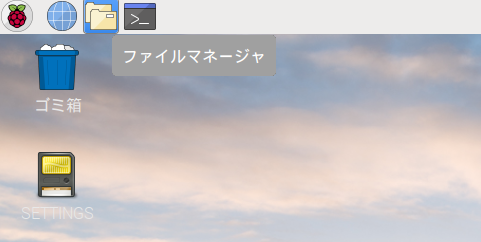
\includegraphics[keepaspectratio, height=30mm]{../../asset/image/textbook-img032.png}
    \vss}
    \vspace{40mm}
  \end{minipage}
  %

  \begin{minipage}[t]{0.49\linewidth}
    \textcircled{\scriptsize{2}}\\
    ファイルマネージャが開いて、自分のフォルダの中が\ruby{表示}{ひょうじ}されます。
    （ウィンドウの色が\ruby{違}{ちが}うかもしれませんが、色はあとで変えられます。）
  \end{minipage}\hfill
  %
  \begin{minipage}[t]{0.49\linewidth}
    \centering
    \vbox to 0pt{\vskip-3mm
      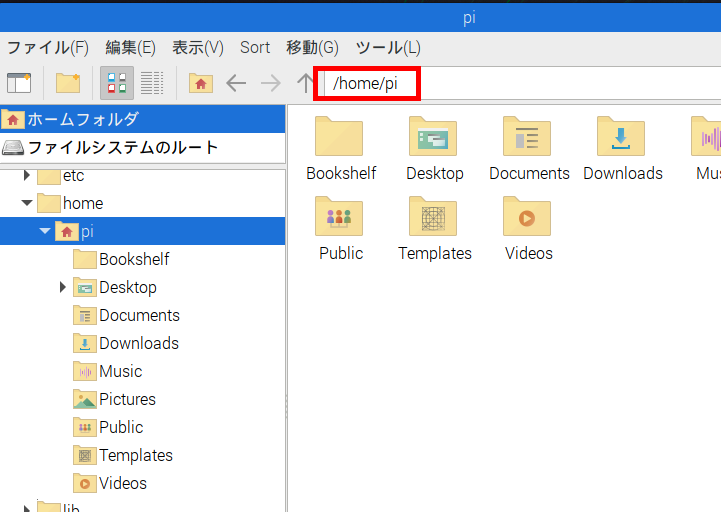
\includegraphics[keepaspectratio, height=50mm]{../../asset/image/textbook-img1020.png}
    \vss}
    \vspace{60mm}
  \end{minipage}



ファイルマネージャのウィンドウの左側には、フォルダがツリー\ruby{表示}{ひょうじ}されます。
右側には、ツリーで選択されているフォルダ内のファイルが\ruby{表示}{ひょうじ}されます。
ファイルマネージャは、\ruby{起動}{きどう}すると、\ruby{最初}{さいしょ}に自分のフォルダを\ruby{表示}{ひょうじ}します。
赤\ruby{枠}{わく}で囲まれたところに、自分のフォルダのパスが書いてあります。
パスについての\ruby{詳}{くわ}しい説明は、\ruby{以降}{いこう}の回で出てくるので、
今はとりあえずフォルダ、ファイルの「住所」と考えてください。
この例では、\verb|/home/pi|と表示されていますが、みなさんの場合は\ruby{違}{ちが}うパスが表示されていると思います。
\textbf{\color{red}ここには、最初に\ruby{設定}{せってい}した「ユーザ名」が反映されます。}
例えば、「\verb|chiba|」というユーザ名を\ruby{設定}{せってい}した場合は、赤\ruby{枠}{わく}の中に、
\verb|/home/chiba| と表示されます。
\vspace{20pt}

\begin{tcolorbox}[title=\useOmetoi,breakable]
  自分のフォルダのパスを見てみよう。
  \begin{enumerate}
    \addquiz{自分のフォルダのパスを下の\ruby{記入欄}{きにゅうらん}に記入してみましょう。}
  \end{enumerate}
\end{tcolorbox}
\clearpage



%
% subsubsection 2
%
\subsubsection{フォルダを作成しよう}
\hrule\vspace*{5mm}

\texttt{Documents}フォルダの中に\texttt{taro}という名前のフォルダを作成しましょう。\\

{\bf 作成する手順}

% \begin{figure}[H]
  \begin{minipage}[t]{0.44\columnwidth}
    % \vspace*{-30mm}
    \textcircled{\scriptsize{1}}\\
    ウィンドウマネージャの左側で、自分のフォルダの中の\texttt{Documents}フォルダをクリックした後、
    右側の空白部分で右クリックして、「New Folder」にカーソルを合わせてクリックする
  \end{minipage}\hfill
  %
  \begin{minipage}[t]{0.55\columnwidth}
    \centering
    \vbox to 0pt{\vskip-3mm
      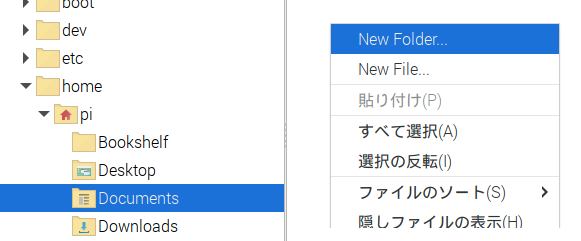
\includegraphics[keepaspectratio, height=35mm]{../../asset/image/textbook-img034x.png}
    \vss}
    \vspace{45mm}
  \end{minipage}
  %
% \end{figure}
%

\begin{minipage}[t]{0.44\columnwidth}
  \textcircled{\scriptsize{2}}\\
  フォルダの新規作成ウィンドウが表示されるので、テキストボックスに作成したいフォルダの名前（\texttt{taro}）を入力してOKをクリックする
\end{minipage}\hfill
%
\begin{minipage}[t]{0.55\columnwidth}
  \centering
  \vbox to 0pt{\vskip-3mm
    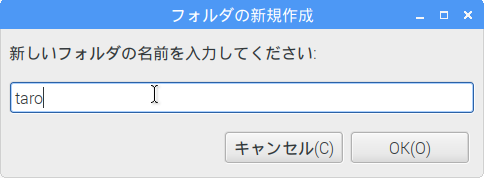
\includegraphics[keepaspectratio, height=30mm]{../../asset/image/textbook-img039x.png}
  \vss}
  \vspace{40mm}
\end{minipage}
%

\begin{minipage}[t]{0.44\columnwidth}
  \textcircled{\scriptsize{3}}\\
  入力した名前（\texttt{taro}）のフォルダが作成できていることを確認しよう
\end{minipage}\hfill
%
\begin{minipage}[t]{0.55\columnwidth}
  \centering
  \vbox to 0pt{\vskip-3mm
    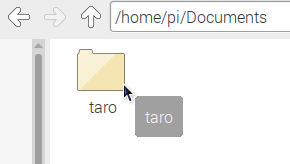
\includegraphics[keepaspectratio, height=30mm]{../../asset/image/textbook-img040x.png}
  \vss}
  \vspace{40mm}
\end{minipage}
%
% \end{figure}
%

たくさんのファイルをあつかう場合、フォルダはとても大切です。
フォルダには、\ruby{画像}{がぞう}やプログラムのコードなど、いろいろなファイルを\ruby{保存}{ほぞん}しておきますので、
わかりやすく\ruby{関係性}{かんけいせい}のある名前を付けてあげましょう。
なお、ファイルやフォルダの名前には、プログラムからあつかいやすいように、空白の入らない半角のアルファベットを使いましょう。
\vspace{20pt}

\begin{tcolorbox}[title=\useOmetoi,breakable]
  \begin{enumerate}
    \addex{\texttt{Desktop}フォルダの中に、\texttt{space1}という名前のフォルダを作りましょう。}
    \addex{\texttt{Desktop}フォルダの中に、\texttt{space2}という名前のフォルダを作りましょう。}
  \end{enumerate}

\end{tcolorbox}


%
% subsubsection 3
%
\subsubsection{フォルダを\ruby{移動}{いどう}しよう}
\hrule\vspace*{5mm}

まずは、\texttt{Desktop}フォルダの中にある\texttt{space1}フォルダの中に、新しく\texttt{move}フォルダを作ります。
そして、この\texttt{move}フォルダを\texttt{space2}フォルダの中に移動します。
（\texttt{space1}と\texttt{space2}は、直前の問題で作成したフォルダです。）\\

{\bf フォルダを移動する手順}

\begin{minipage}[t]{0.49\columnwidth}
  \textcircled{\scriptsize{1}}\\
  ウィンドウ左側の\texttt{Desktop}をクリックして、\texttt{space1}と\texttt{space2}フォルダがあることを確認する（フォルダがない時は、作成してください）
\end{minipage}\hfill
%
\begin{minipage}[t]{0.49\columnwidth}
  \centering
  \vbox to 0pt{\vskip-3mm
    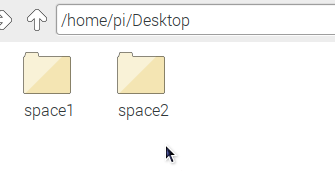
\includegraphics[keepaspectratio, height=30mm]{../../asset/image/textbook-img051.png}
  \vss}
  \vspace{35mm}
\end{minipage}


\begin{minipage}[t]{0.49\columnwidth}
  \textcircled{\scriptsize{2}}\\
  \texttt{sapce1}をダブルクリックして\texttt{space1}の中に移動し、\texttt{move}フォルダを作成する
\end{minipage}\hfill
%
\begin{minipage}[t]{0.49\columnwidth}
  \centering
  \vbox to 0pt{\vskip-3mm
    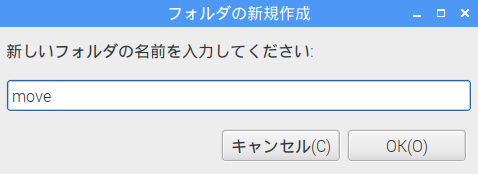
\includegraphics[keepaspectratio, height=25mm]{../../asset/image/textbook-img050.png}
  \vss}
  \vspace{35mm}
\end{minipage}


\begin{minipage}[t]{0.49\columnwidth}
  \textcircled{\scriptsize{3}}\\
  \texttt{move}フォルダ上で右クリックして、メニューから切り取りをクリックする
\end{minipage}\hfill
%
\begin{minipage}[t]{0.49\columnwidth}
  \centering
  \vbox to 0pt{\vskip-3mm
    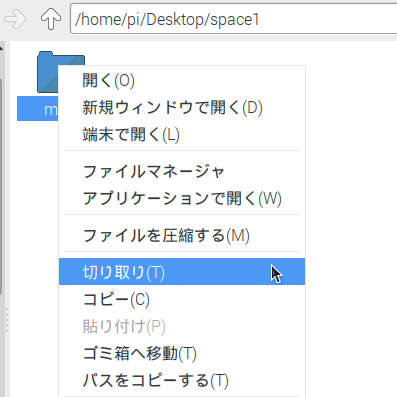
\includegraphics[keepaspectratio, height=55mm]{../../asset/image/textbook-img048x.png}
  \vss}
  \vspace{60mm}
\end{minipage}


\begin{minipage}[t]{0.49\columnwidth}
  \textcircled{\scriptsize{4}}\\
  \texttt{sapce2}をダブルクリックして\texttt{space2}の中に移動し、右側の空白部分で右クリックして、メニューから\ruby{貼}{は}り付けをクリックする
\end{minipage}\hfill
%
\begin{minipage}[t]{0.49\columnwidth}
  \centering
  \vbox to 0pt{\vskip-3mm
    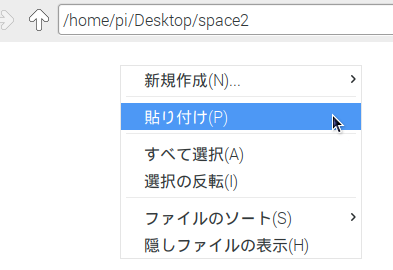
\includegraphics[keepaspectratio, height=40mm]{../../asset/image/textbook-img046xx.png}
  \vss}
  \vspace{45mm}
\end{minipage}


\begin{minipage}[t]{0.49\columnwidth}
  \textcircled{\scriptsize{5}}\\
  これで、\texttt{space1}の中にあった\texttt{move}フォルダが\texttt{sapce2}の中に移動しました
\end{minipage}\hfill
%
\begin{minipage}[t]{0.49\columnwidth}
  \centering
  \vbox to 0pt{\vskip-3mm
  \vss}
  \vspace{20mm}
\end{minipage}

\begin{tcolorbox}[title=\useOmetoi,breakable]
  \begin{enumerate}
    \addex{\texttt{space1}フォルダの中に、\texttt{rasp}という名前のフォルダを作り、さらにそのフォルダ内に\texttt{berry}という名前のフォルダを作成しよう。}
    \addex{\texttt{rasp}フォルダを\texttt{space2}フォルダの中に移動して、その中身を確認しよう。}
  \end{enumerate}

\end{tcolorbox}



%
% subsubsection 4
%
\subsubsection{ファイル名・フォルダ名を\ruby{変更}{へんこう}しよう}
\hrule\vspace*{5mm}


\texttt{before}という名前のフォルダを\texttt{Documents}直下に作り、作成した後でそのフォルダ名を\texttt{after}に変えよう。
ファイル名もフォルダ名も同じ手順で変えることができます。
これは、間違えたファイル名・フォルダ名を変えたいときなどに使います。\\

{\bf ファイル名・フォルダを変更する手順}

\begin{minipage}[t]{0.49\columnwidth}
  \textcircled{\scriptsize{1}}\\
  ウィンドウ左側の\texttt{Documents}をクリックして、\texttt{before}フォルダを作成する
\end{minipage}\hfill
%
\begin{minipage}[t]{0.49\columnwidth}
  \centering
  \vbox to 0pt{\vskip-3mm
    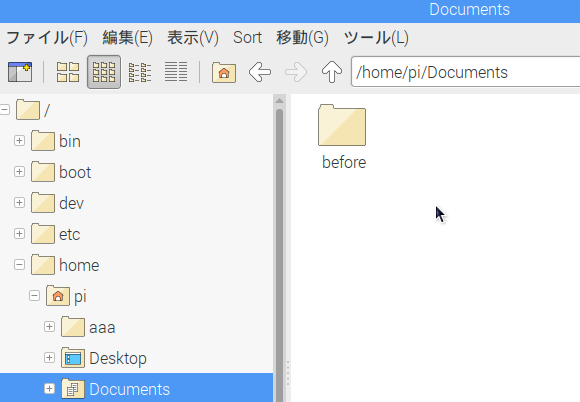
\includegraphics[keepaspectratio, height=45mm]{../../asset/image/textbook-img058.png}
  \vss}
  \vspace{50mm}
\end{minipage}

\begin{minipage}[t]{0.49\columnwidth}
  \textcircled{\scriptsize{2}}\\
  \texttt{before}フォルダ上で右クリックして、メニューからファイル名の変更をクリック
\end{minipage}\hfill
%
\begin{minipage}[t]{0.49\columnwidth}
  \centering
  \vbox to 0pt{\vskip-3mm
    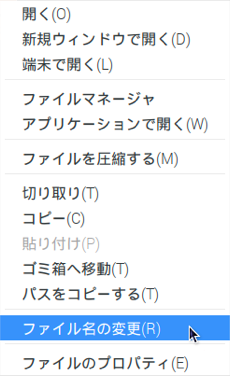
\includegraphics[keepaspectratio, height=45mm]{../../asset/image/textbook-img057x.png}
  \vss}
  \vspace{50mm}
\end{minipage}

\begin{minipage}[t]{0.49\columnwidth}
  \textcircled{\scriptsize{3}}\\
  名前を\texttt{after}に変更してOKをクリック
\end{minipage}\hfill
%
\begin{minipage}[t]{0.49\columnwidth}
  \centering
  \vbox to 0pt{\vskip-3mm
    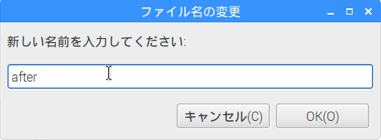
\includegraphics[keepaspectratio, height=25mm]{../../asset/image/textbook-img055x.png}
  \vss}
  \vspace{30mm}
\end{minipage}

\begin{tcolorbox}[title=\useOmetoi,breakable]
  \begin{enumerate}
    \addex{\texttt{Documents}フォルダの中に、\texttt{wrong}という名前のフォルダを作り、その後でフォルダ名を\texttt{correct}に変えよう。}
  \end{enumerate}
\end{tcolorbox}
\clearpage

%
% subsection 1.2.2
%
\subsection{文字の入力}

テキストエディタを開き、アルファベットをa〜zまで入力しましょう。
その後で、「こんにちは」「こんばんは」「ごきげんよう」「さようなら」「ありがとう」をそれぞれ一行に入力しましょう。
日本語を入力するときには、英字入力モードから日本語入力モードに切り\ruby{替}{か}える必要があります。
英字入力と日本語入力のモードを切り\ruby{替}{か}えるには、下図の赤わくで囲んだCtrlキーとスペースキーを同時に\ruby{押}{お}します。

\begin{figure}[hb]
  \centering
    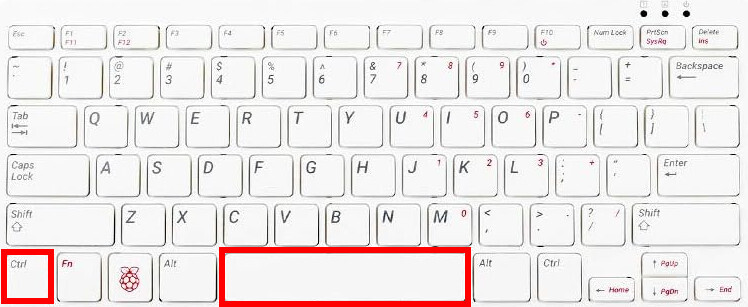
\includegraphics[keepaspectratio, height=40mm]{../../asset/image/2024_keyboard.jpg}
    \caption{入力モードの切り替え}
    \label{fig:20}
\end{figure}




{\bf 文字入力の手順}

\begin{minipage}[t]{0.49\columnwidth}
  \textcircled{\scriptsize{1}}\\
  左上のラズベリーのアイコンをクリックして表示されるメニューから、[アクセサリ]->[Text Editor]をクリックします
\end{minipage}\hfill
%
\begin{minipage}[t]{0.49\columnwidth}
  \centering
  \vbox to 0pt{\vskip-3mm
    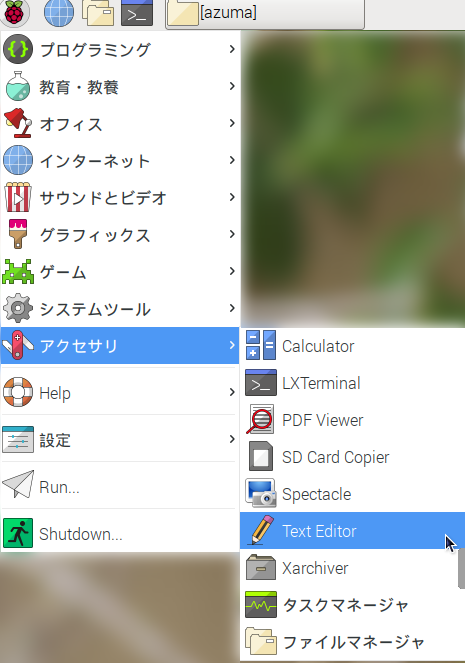
\includegraphics[keepaspectratio, height=45mm]{../../asset/image/textbook-img064x.png}
  \vss}
  \vspace{50mm}
\end{minipage}

\begin{minipage}[t]{0.49\columnwidth}
  \textcircled{\scriptsize{2}}\\
  テキストエディタのウィンドウをクリックして、左上（右図の赤線）のカーソルが\ruby{点滅}{てんめつ}していることを確認してください
\end{minipage}\hfill
%
\begin{minipage}[t]{0.49\columnwidth}
  \centering
  \vbox to 0pt{\vskip-3mm
    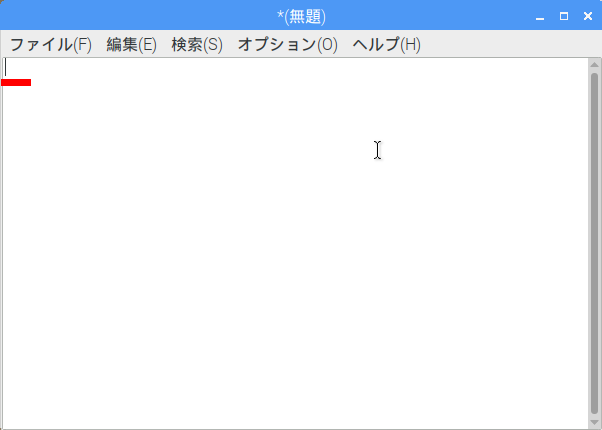
\includegraphics[keepaspectratio, height=40mm]{../../asset/image/textbook-img063.png}
  \vss}
  \vspace{45mm}
\end{minipage}

\begin{minipage}[t]{0.49\columnwidth}
  \textcircled{\scriptsize{3}}\\
  Ctrlキーを\ruby{押}{お}しながらスペースキーを\ruby{押}{お}して文字入力を切り替えよう
  （タスクバーの右上のアイコンが、英字入力の場合は「キーボード」アイコンに、日本語入力の場合は「あ」アイコンに\ruby{替}{か}わります）
\end{minipage}\hfill
%
\begin{minipage}[t]{0.49\columnwidth}
  \centering
  \vbox to 0pt{\vskip-3mm
    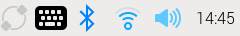
\includegraphics[scale=0.8]{../../asset/image/textfig_001.png}
    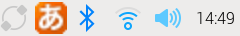
\includegraphics[scale=0.8]{../../asset/image/textfig_002.png}
  \vss}
  \vspace{35mm}
\end{minipage}

\begin{minipage}[t]{0.49\columnwidth}
  \textcircled{\scriptsize{4}}\\
  まずはアルファベットを入力したいので、「キーボード」アイコンに切り\ruby{替}{か}えて、a～zまで入力しよう
\end{minipage}\hfill
%
\begin{minipage}[t]{0.49\columnwidth}
  \centering
  \vbox to 0pt{\vskip-3mm
    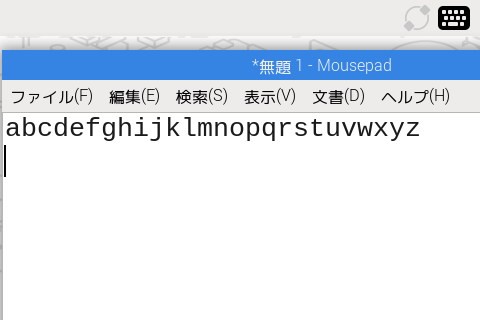
\includegraphics[scale=0.5]{../../asset/image/textfig_003.png}
  \vss}
  \vspace{45mm}
\end{minipage}

\begin{minipage}[t]{0.49\columnwidth}
  \textcircled{\scriptsize{5}}\\
  次に日本語を入力したいので、「あ」アイコンに切り\ruby{替}{か}えて、こんにちは～ありがとうまでを入力しよう
\end{minipage}\hfill
%
\begin{minipage}[t]{0.49\columnwidth}
  \centering
  \vbox to 0pt{\vskip-3mm
    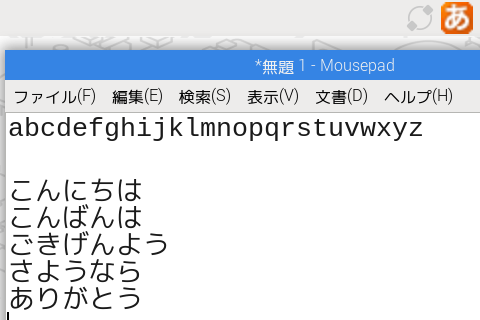
\includegraphics[scale=0.5]{../../asset/image/textfig_004.png}
  \vss}
  \vspace{45mm}
\end{minipage}

\begin{tcolorbox}[title=\useOmetoi,breakable]
  \begin{enumerate}
    \addex{テキストエディタで\texttt{A}～\texttt{Z}を入力しよう（ヒント：大文字を入力するにはshiftキーを\ruby{押}{お}しながらアルファベットキーを打つ）。}
  \end{enumerate}
\end{tcolorbox}


%
% subsubsection 1
%
\subsubsection{半角文字と全角文字について}
\hrule\vspace*{5mm}

全角文字とは、文字の縦と横の比率が1対1の文字のことを指します。
それに対して、半角文字は、横の幅が全角の半分（縦と横の比率が2対1）になります。
それでは、全角と半角の文字の違いを見てみましょう。


\begin{figure}[hb]
  \centering
    % 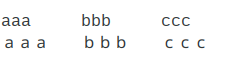
\includegraphics[keepaspectratio, height=20mm]{../../asset/image/textbook-img066.png}
    % 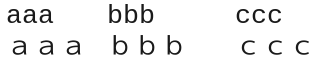
\includegraphics[keepaspectratio, width=0.5\columnwidth]{../../asset/image/textfig_005.png}
    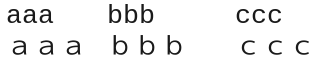
\includegraphics[scale=0.8]{../../asset/image/textfig_005.png}
    \caption{半角文字と全角文字（上：半角，下：全角）}
    \label{fig:21}
\end{figure}

\noindent%
ここで、上の行が半角で下の行が全角の例になります。
アルファベットのサイズからも分かる通り、横幅が大きい方が全角で、小さい方が半角だと覚えておいてください。
日本語の文字は（半角カタカナを除いて）すべて全角です。
なお、
\textbf{\color{red}{プログラミングでアルファベットや記号を入力するときは、必ず半角文字(小さい文字)を使いましょう}}。
\clearpage


%
% subsubsection 1
%
\subsubsection{ブラウザで\ruby{検索}{けんさく}しよう}
\hrule\vspace*{5mm}

ウェブブラウザ（ブラウザとも呼ばれます）を開いていろいろなことを\ruby{検索}{けんさく}してみましょう。
ブラウザを使用するとウェブサイトを開くことができます。
もし、困ったことがあったら自分で\ruby{検索}{けんさく}できるように使い方を覚えておきましょう。\\

{\bf \ruby{検索}{けんさく}の手順}

\begin{minipage}[t]{0.49\columnwidth}
  \textcircled{\scriptsize{1}}\\
  デスクトップ左上の地球儀のアイコンをクリックするとブラウザが起動します
\end{minipage}\hfill
%
\begin{minipage}[t]{0.49\columnwidth}
  \centering
  \vbox to 0pt{\vskip-3mm
    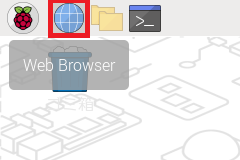
\includegraphics[scale=0.8]{../../asset/image/textfig_006.png}
  \vss}
  \vspace{35mm}
\end{minipage}

\begin{minipage}[t]{0.49\columnwidth}
  \textcircled{\scriptsize{2}}\\
  ブラウザが起動したら、赤で囲われている部分をクリックし、キーボードで\ruby{検索}{けんさく}したいワードを入力して
  Enterキーを押します
\end{minipage}\hfill
%
\begin{minipage}[t]{0.49\columnwidth}
  \centering
  \vbox to 0pt{\vskip-3mm
    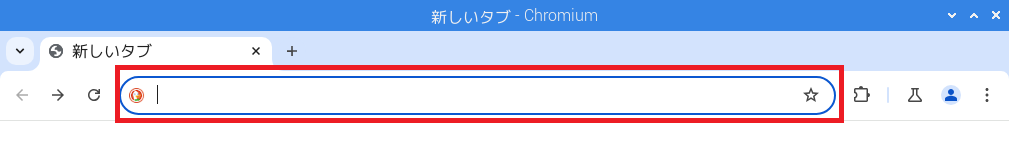
\includegraphics[scale=0.25]{../../asset/image/textfig_007.png}
  \vss}
  \vspace{20mm}
\end{minipage}
\vspace*{10mm}


{\bf 画像の\ruby{検索}{けんさく}}（「ねこ」の画像を\ruby{検索}{けんさく}してみよう）

\begin{minipage}[t]{0.49\columnwidth}
  \textcircled{\scriptsize{1}}\\
  ブラウザを起動して、「ねこ」と入力してEnterキーを押すと、「ねこ」の\ruby{検索}{けんさく}結果が表示されます
  % （著作権の関画像をぼかしています）
\end{minipage}\hfill
%
\begin{minipage}[t]{0.49\columnwidth}
  \centering
  \vbox to 0pt{\vskip-3mm
    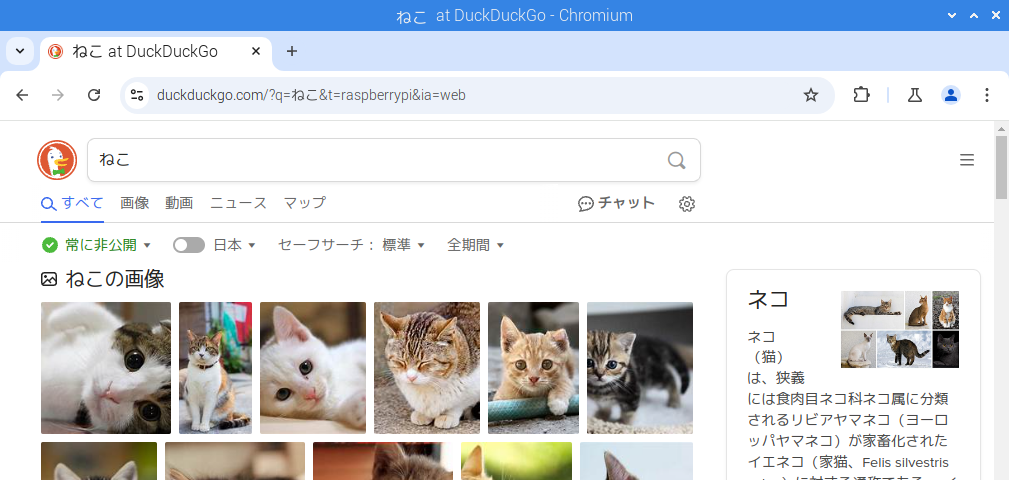
\includegraphics[scale=0.25]{../../asset/image/textfig_008.png}
  \vss}
  \vspace{40mm}
\end{minipage}

\begin{minipage}[t]{0.49\columnwidth}
  \textcircled{\scriptsize{2}}\\
  赤線で囲まれている「画像」をクリックすると、「ねこ」の画像だけが\ruby{検索}{けんさく}できます
  （「すべて」をクリックすると、もとの\ruby{検索}{けんさく}結果にもどります）
\end{minipage}\hfill
%
\begin{minipage}[t]{0.49\columnwidth}
  \centering
  \vbox to 0pt{\vskip-3mm
    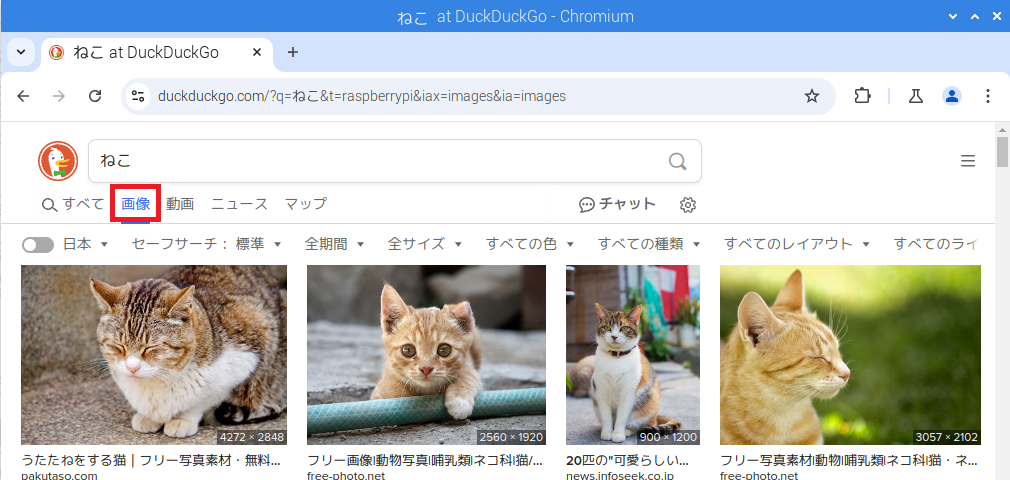
\includegraphics[scale=0.25]{../../asset/image/textfig_009x.png}
  \vss}
  \vspace{45mm}
\end{minipage}

\begin{tcolorbox}[title=\useOmetoi,breakable]
  \begin{enumerate}
    \addex{自分の好きなキーワードで\ruby{検索}{けんさく}してみよう。}
  \end{enumerate}
\end{tcolorbox}



%
% subsubsection 2
%
\subsubsection{キーボード入力の練習をしよう}
\hrule\vspace*{5mm}

キーボードで文字を入力することをタイピングと言います。
ここでは、タイピング練習ができるウェブサイト「e-typing」を使って、タイピングに\ruby{慣}{な}れましょう。
なお、パソコンで日本語を入力するときは、ローマ字入力が基本ですので、不慣れな場合は、
下のローマ字・アルファベット表で入力方法を確認してください。

\begin{figure}[hb]
  \centering
    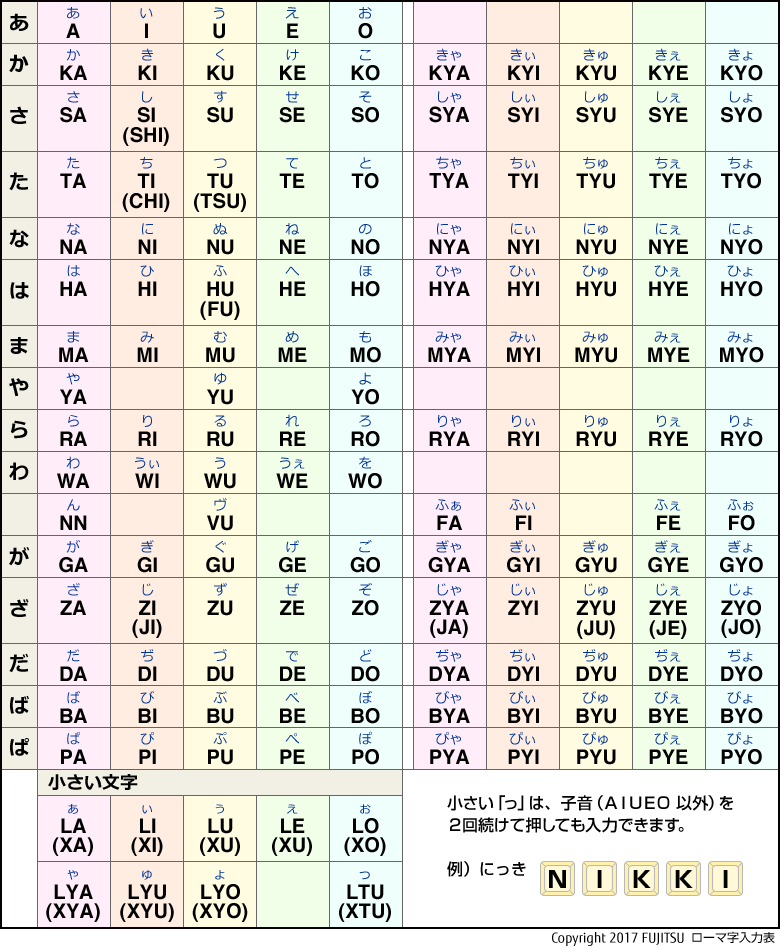
\includegraphics[scale=0.4]{../../asset/image/textbook-img080.png}
    \caption{ローマ字・アルファベット表}
    \label{fig:22}
\end{figure}

{\bf タイピング練習の手順}

\begin{minipage}[t]{0.49\columnwidth}
  \textcircled{\scriptsize{1}}\\
  ブラウザで「etyping」を\ruby{検索}{けんさく}して、タイピング練習ができるウェブサイト
  「e-typing」をみつけましょう（右図のように\ruby{検索}{けんさく}できたら、
  赤わくのリンクをクリックしてください）
\end{minipage}\hfill
%
\begin{minipage}[t]{0.49\columnwidth}
  \centering
  \vbox to 0pt{\vskip-3mm
    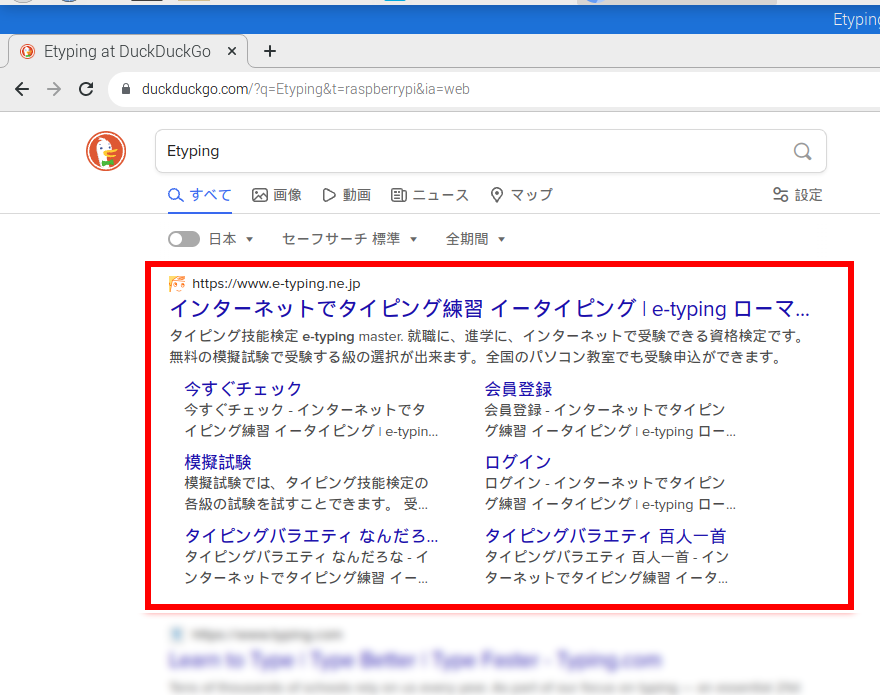
\includegraphics[scale=0.3]{../../asset/image/textbook-img086x.png}
  \vss}
  \vspace{35mm}
\end{minipage}

\begin{minipage}[t]{0.49\columnwidth}
  \textcircled{\scriptsize{2}}\\
  右図のようにホームページが開けたら、「今すぐチェック！」ボタンをクリックしましょう
\end{minipage}\hfill
%
\begin{minipage}[t]{0.49\columnwidth}
  \centering
  \vbox to 0pt{\vskip-3mm
    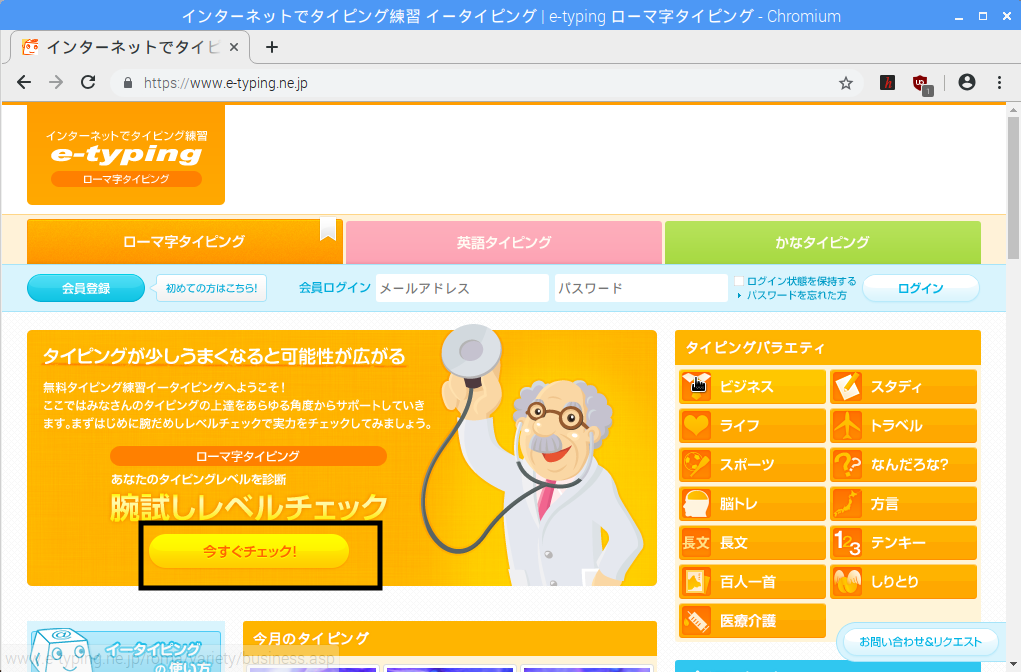
\includegraphics[scale=0.27]{../../asset/image/textbook-img087.png}
  \vss}
  \vspace{50mm}
\end{minipage}

\begin{minipage}[t]{0.49\columnwidth}
  \textcircled{\scriptsize{3}}\\
  もう一度「今すぐチェック！」ボタンをクリックすると、右図のような
  \ruby{腕試}{うでだめ}しレベルチェックウィンドウが表示されますので、
  スタートボタンをクリックします
\end{minipage}\hfill
%
\begin{minipage}[t]{0.49\columnwidth}
  \centering
  \vbox to 0pt{\vskip-3mm
    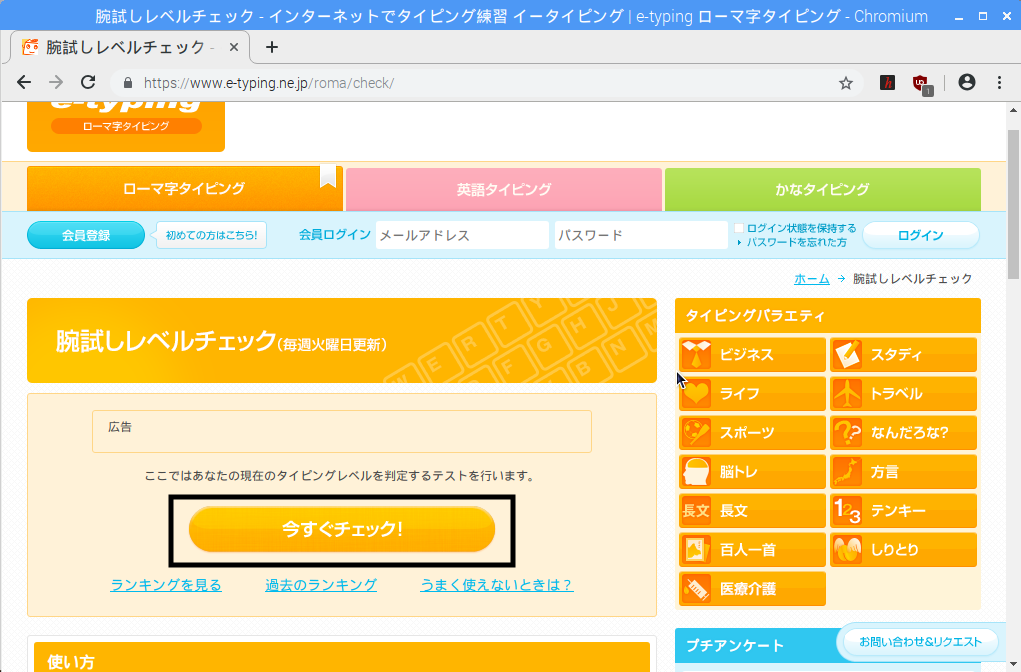
\includegraphics[scale=0.27]{../../asset/image/textbook-img088.png}
  \vss}
  \vspace{50mm}
\end{minipage}

\begin{minipage}[t]{0.49\columnwidth}
  \textcircled{\scriptsize{4}}\\
  キーボードのスペースキーを押すとゲームがスタートします
\end{minipage}\hfill
%
\begin{minipage}[t]{0.49\columnwidth}
  \centering
  \vbox to 0pt{\vskip-3mm
    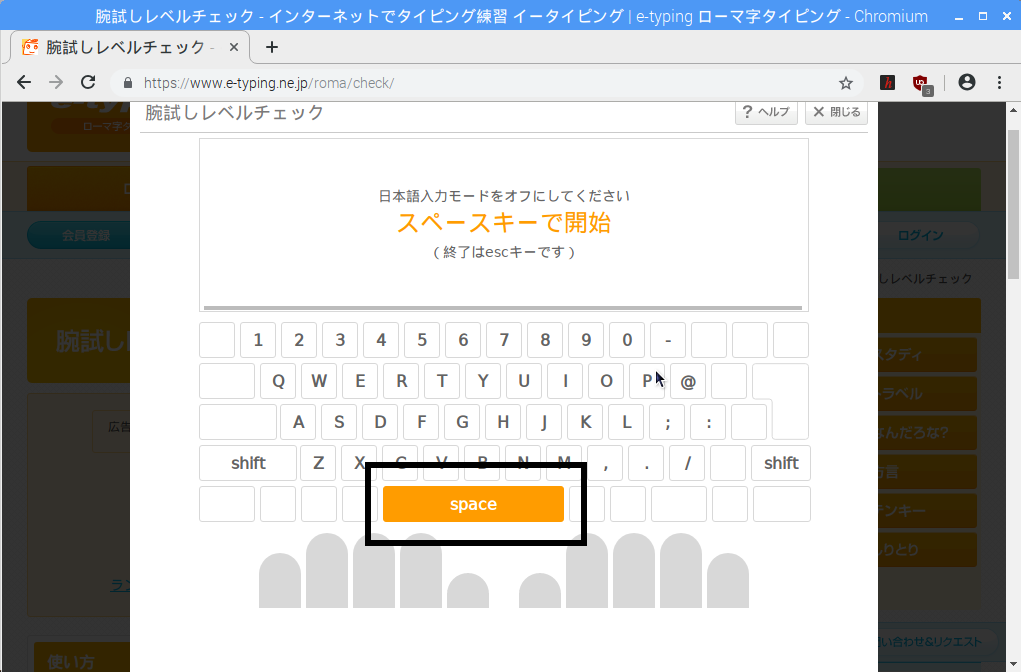
\includegraphics[scale=0.27]{../../asset/image/textbook-img090.png}
  \vss}
  \vspace{50mm}
\end{minipage}

\begin{minipage}[t]{0.49\columnwidth}
  \textcircled{\scriptsize{5}}\\
  ゲームでは、画面左上の文字をキーボードで入力します\\
  キーの位置は画面中央のキーボードにオレンジ色で表示されます\\
  \ruby{慣}{な}れてきたら、画面下のオレンジ色の指で、オレンジ色のキーを\ruby{押}{お}せるように練習してみましょう
\end{minipage}\hfill
%
\begin{minipage}[t]{0.49\columnwidth}
  \centering
  \vbox to 0pt{\vskip-3mm
    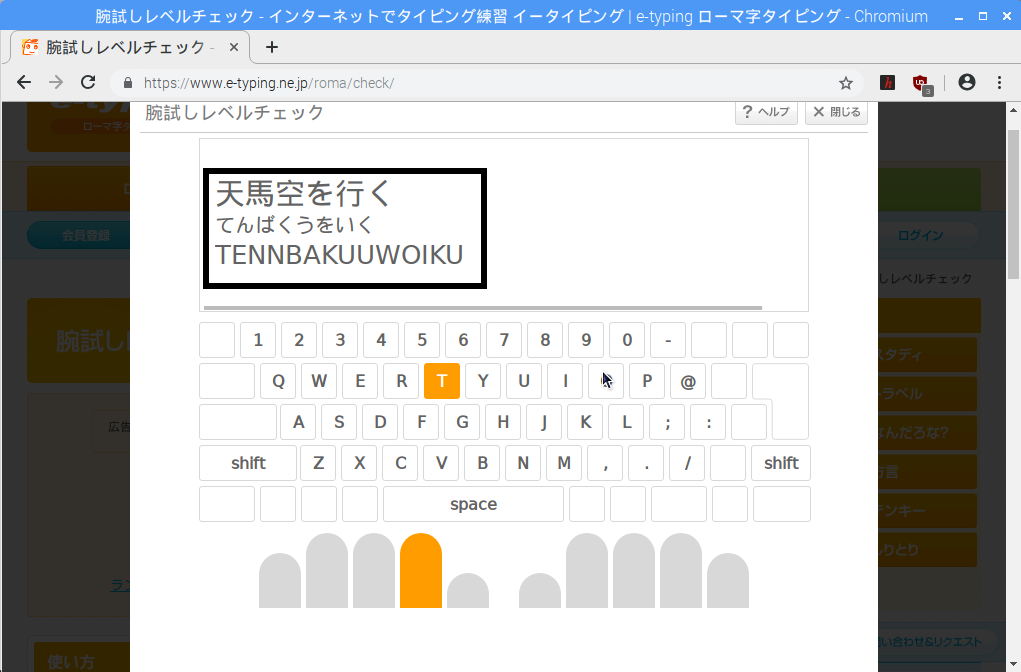
\includegraphics[scale=0.27]{../../asset/image/textbook-img089.png}
  \vss}
  \vspace{50mm}
\end{minipage}
\clearpage



%
% subsection 1.3
%
\subsection{画面の見た目を自分の好みに変えよう}

ここでは、ラズパイのデスクトップに表示される画像（かべ紙）やウィンドウの色などを変えてみましょう。

%
% subsubsection 1
%
\subsubsection{画像を\ruby{検索}{けんさく}して、目当ての画像を保存しよう}
\hrule\vspace*{5mm}

ブラウザで\ruby{検索}{けんさく}した\ruby{画像}{がぞう}は、ラズパイのフォルダ内に\ruby{保存}{ほぞん}することができます。
フォルダ名は、中に入っている\ruby{画像}{がぞう}やファイルに関連する名前にすると、
どんな\ruby{画像}{がぞう}やファイルが\ruby{保存}{ほぞん}されているか分かりやすくなります。
ここでは、\texttt{Pictures}フォルダの中に\texttt{usagi}フォルダを作成して、
その中に\ruby{画像検索}{がぞうけんさく}で見つけたうさぎの\ruby{画像}{がぞう}を\ruby{保存}{ほぞん}しましょう。\\

{\bf 手順}

\begin{minipage}[t]{0.49\columnwidth}
  \textcircled{\scriptsize{1}}\\
  ファイルマネージャを使って、\texttt{Pictures}フォルダの中に\texttt{usagi}フォルダを作成しましょう
\end{minipage}\hfill
%
\begin{minipage}[t]{0.49\columnwidth}
  \centering
  \vbox to 0pt{\vskip-3mm
    % 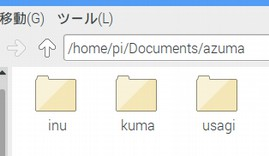
\includegraphics[scale=0.3]{../../asset/image/textbook-img094.jpg}
    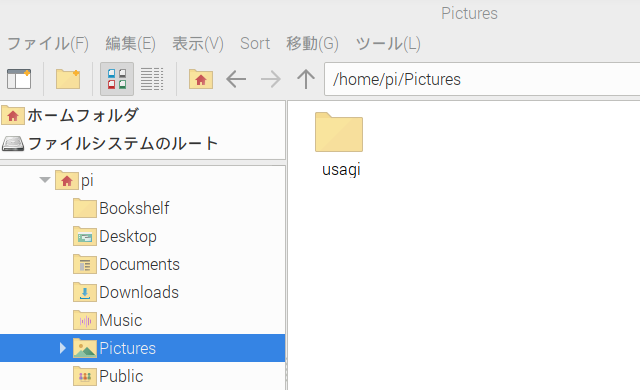
\includegraphics[width=0.8\linewidth]{../../asset/image/textbook-img094x.png}
  \vss}
  \vspace{45mm}
\end{minipage}

\begin{minipage}[t]{0.49\columnwidth}
  \textcircled{\scriptsize{2}}\\
  ブラウザを使って「うさぎ」の\ruby{画像}{がぞう}を\ruby{検索}{けんさく}しましょう。
  目当ての画像を見つけたらクリックして大きく表示します
\end{minipage}\hfill
%
\begin{minipage}[t]{0.49\columnwidth}
  \centering
  \vbox to 0pt{\vskip-3mm
    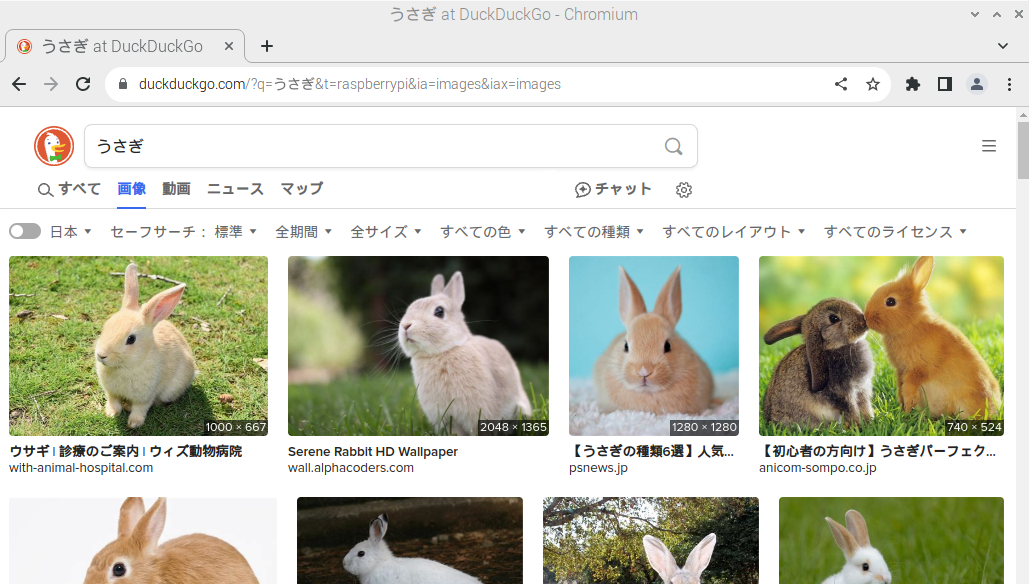
\includegraphics[height=0.5\linewidth]{../../asset/image/textbook-img096x.png}
  \vss}
  \vspace{45mm}
\end{minipage}

\begin{minipage}[t]{0.49\columnwidth}
  \textcircled{\scriptsize{3}}\\
  \ruby{画像}{がぞう}の上で右クリックしてメニューを表示し、「名前をつけて画像を保存」をクリックします
\end{minipage}\hfill
%
\begin{minipage}[t]{0.49\columnwidth}
  \centering
  \vbox to 0pt{\vskip-3mm
    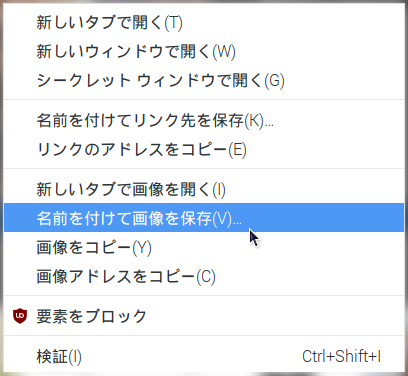
\includegraphics[width=0.6\linewidth]{../../asset/image/textbook-img095x.png}
  \vss}
  \vspace{45mm}
\end{minipage}

\begin{minipage}[t]{0.49\columnwidth}
  \textcircled{\scriptsize{4}}\\
  ウィンドウ左側からPicturesフォルダを選択し、\texttt{usagi}フォルダをダブルクリックして保存場所を指定します。
  上のテキストボックスに名前を入力したら、右下の「保存」をクリックします
  （この例では画像に\texttt{cute.jpg}という名前を付けています）
\end{minipage}\hfill
%
\begin{minipage}[t]{0.49\columnwidth}
  \centering
  \vbox to 0pt{\vskip-3mm
    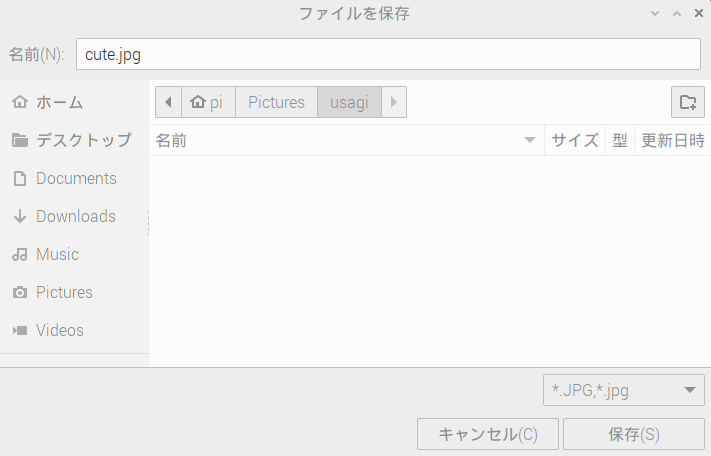
\includegraphics[width=0.8\linewidth]{../../asset/image/textbook-img099x.png}
  \vss}
  \vspace{45mm}
\end{minipage}

\begin{minipage}[t]{0.49\columnwidth}
  \textcircled{\scriptsize{5}}\\
  ファイルマネージャで\texttt{usagi}フォルダを開いて、画像が保存されているか確認しましょう
\end{minipage}\hfill
%
\begin{minipage}[t]{0.49\columnwidth}
  \centering
  \vbox to 0pt{\vskip-3mm
    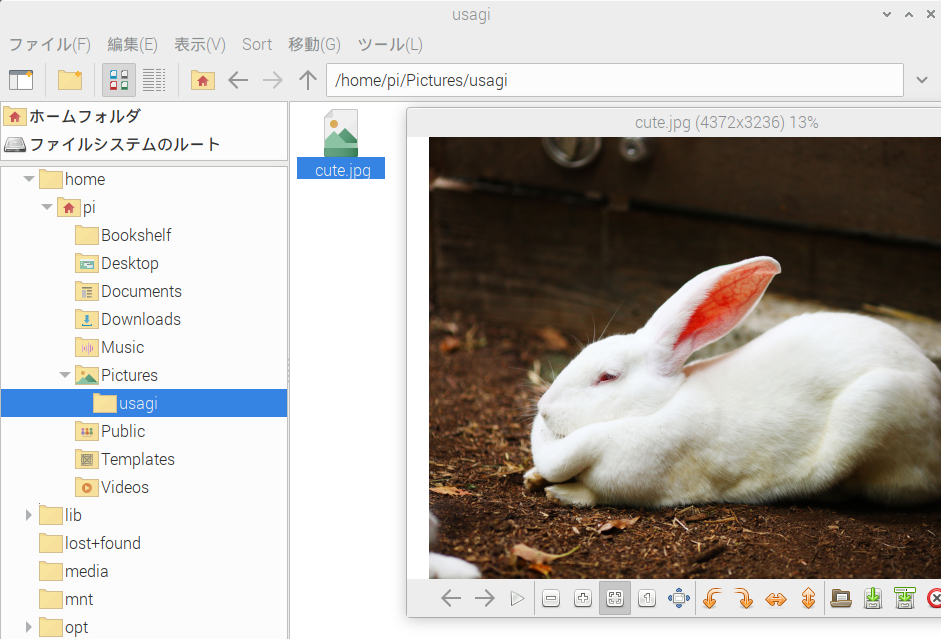
\includegraphics[width=0.8\linewidth]{../../asset/image/textbook-img102x.png}
  \vss}
  \vspace{45mm}
\end{minipage}

\begin{tcolorbox}[title=\useOmetoi,breakable]
  \begin{enumerate}
    \addex{好きな画像を検索して、自分で作成したフォルダの中に保存しよう。}
  \end{enumerate}
\end{tcolorbox}

\clearpage

%
% subsubsection 2
%
\subsubsection{画面の見た目を自分の好きなものに変えよう}
\hrule\vspace*{5mm}

\ruby{保存}{ほぞん}した\ruby{画像}{がぞう}をデスクトップのかべ紙にしてみましょう。
いつも目に入るものなので、自分好みにカスタマイズして気分良く勉強できる\ruby{環境}{かんきょう}にしてみましょう。

{\bf 手順}

\begin{minipage}[t]{0.49\columnwidth}
  \textcircled{\scriptsize{1}}\\
  デスクトップ上で右クリックして、デスクトップの\ruby{設定}{せってい}をクリックします
\end{minipage}\hfill
%
\begin{minipage}[t]{0.49\columnwidth}
  \centering
  \vbox to 0pt{\vskip-3mm
    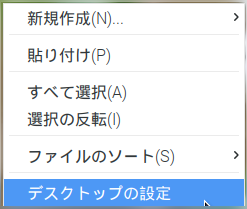
\includegraphics[width=0.5\linewidth]{../../asset/image/textbook-img107x.png}
  \vss}
  \vspace{45mm}
\end{minipage}

\begin{minipage}[t]{0.49\columnwidth}
  \textcircled{\scriptsize{2}}\\
  外観の設定ウィンドウで、右の図の場所をクリックします
\end{minipage}\hfill
%
\begin{minipage}[t]{0.49\columnwidth}
  \centering
  \vbox to 0pt{\vskip-3mm
    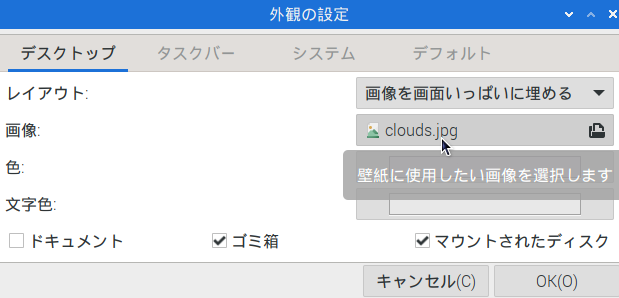
\includegraphics[width=0.8\linewidth]{../../asset/image/textbook-img108.png}
  \vss}
  \vspace{45mm}
\end{minipage}

\begin{minipage}[t]{0.49\columnwidth}
  \textcircled{\scriptsize{3}}\\
  デスクトップに設定したい画像を選びましょう
\end{minipage}\hfill
%
\begin{minipage}[t]{0.49\columnwidth}
  \centering
  \vbox to 0pt{\vskip-3mm
    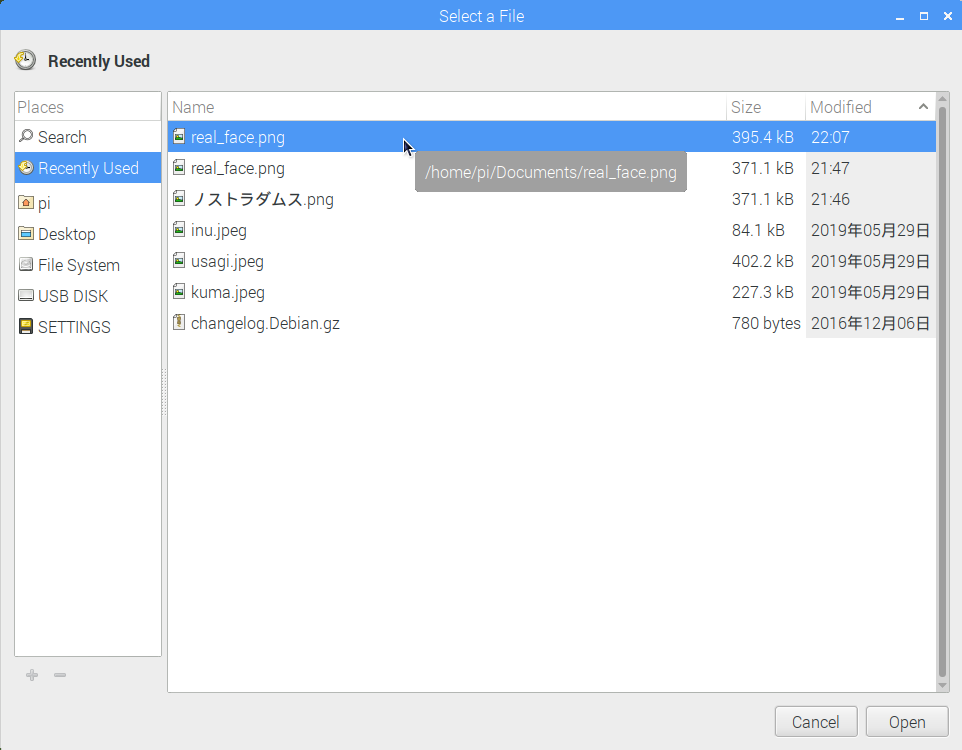
\includegraphics[width=0.8\linewidth]{../../asset/image/textbook-img110.png}
  \vss}
  \vspace{55mm}
\end{minipage}


\begin{tcolorbox}[title=\useOmetoi,breakable]
  \begin{enumerate}
    \addex{デスクトップの壁紙を好きな画像に変えてみましょう。画像はブラウザで検索してください。}
    % \addex{\texttt{Documents}フォルダの中に、\texttt{wrong}という名前のフォルダを作り、その後でフォルダ名を\texttt{correct}に変えよう。}
  \end{enumerate}
\end{tcolorbox}

\clearpage

%
% subsubsection 3
%
\subsubsection{ウィンドウの色を変えてみよう}
\hrule\vspace*{5mm}

ウィンドウの色も、デスクトップと同じように変えることができます。

{\bf 手順}

\begin{minipage}[t]{0.49\columnwidth}
  \textcircled{\scriptsize{1}}\\
  デスクトップ上で右クリックして、デスクトップの\ruby{設定}{せってい}をクリックします
\end{minipage}\hfill
%
\begin{minipage}[t]{0.49\columnwidth}
  \centering
  \vbox to 0pt{\vskip-3mm
    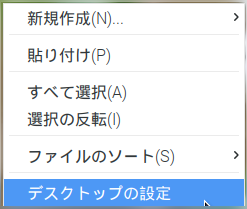
\includegraphics[width=0.5\linewidth]{../../asset/image/textbook-img107x.png}
  \vss}
  \vspace{60mm}
\end{minipage}

\begin{minipage}[t]{0.49\columnwidth}
  \textcircled{\scriptsize{2}}\\
  \ruby{画像}{がぞう}の赤く囲われた「システム」をクリックした後、下の「ハイライト色」をクリックします
\end{minipage}\hfill
%
\begin{minipage}[t]{0.49\columnwidth}
  \centering
  \vbox to 0pt{\vskip-3mm
    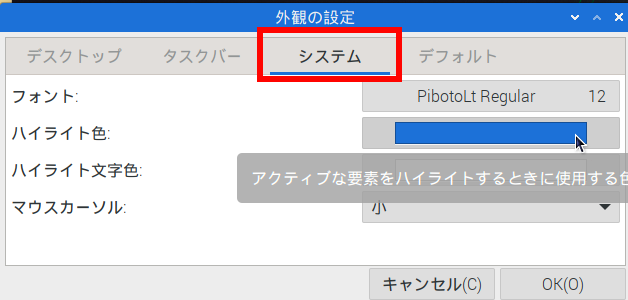
\includegraphics[width=0.8\linewidth]{../../asset/image/textbook-img1001.png}
  \vss}
  \vspace{35mm}
\end{minipage}

\begin{minipage}[t]{0.49\columnwidth}
  \textcircled{\scriptsize{3}}\\
  色の選択ウィンドウから好きな色を選びましょう。
\end{minipage}\hfill
%
\begin{minipage}[t]{0.49\columnwidth}
  \centering
  \vbox to 0pt{\vskip-3mm
    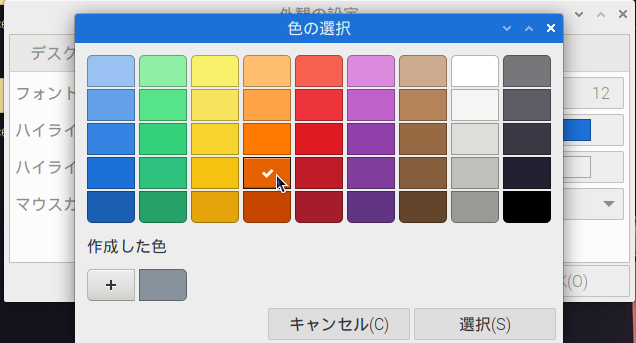
\includegraphics[width=0.8\linewidth]{../../asset/image/textbook-img1002.png}
  \vss}
  \vspace{40mm}
\end{minipage}

\begin{minipage}[t]{0.49\columnwidth}
  \textcircled{\scriptsize{3}}\\
  選び終えると、自動的にウィンドウの色が変わります。
\end{minipage}\hfill
%
\begin{minipage}[t]{0.49\columnwidth}
  \centering
  \vbox to 0pt{\vskip-3mm
    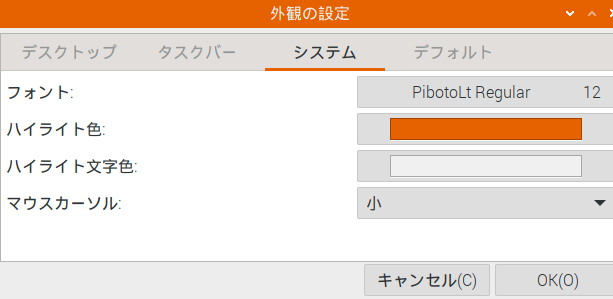
\includegraphics[width=0.8\linewidth]{../../asset/image/textbook-img1003.png}
  \vss}
  \vspace{40mm}
\end{minipage}

\begin{tcolorbox}[title=\useOmetoi,breakable]
  \begin{enumerate}
    \addex{ウィンドウの色を他の色に変えてみましょう。}
  \end{enumerate}
\end{tcolorbox}

\clearpage


\end{document}
